\documentclass[10pt,UKenglish, leqno, xcolor = dvipsnames]{beamer}

\usetheme{UiB}

% Font choice:
\usefonttheme{default}

\usepackage{cite}
\usepackage{amsmath, amsthm, mathtools, color, setspace}
\usepackage{fancyhdr, braket, etoolbox,booktabs,multirow}
\usepackage{xfrac, lmodern, ifsym, bm, multicol, booktabs, pdflscape}
\usepackage[utf8]{inputenx} % For æ, ø, å
\usepackage{csquotes}       % Quotation marks
\usepackage{microtype}      % Improved typography
\usepackage{amssymb}        % Mathematical symbols
\usepackage{mathtools,physics,centernot,tensor}      % Mathematical symbols
\usepackage[absolute, overlay]{textpos} % Arbitrary placement
\setlength{\TPHorizModule}{\paperwidth} % Textpos units
\setlength{\TPVertModule}{\paperheight} % Textpos units
\usepackage[dvipsnames]{xcolor}
\usepackage{tikz}
\usetikzlibrary{tikzmark,calc,overlay-beamer-styles,arrows,shapes}  % Overlay effects for TikZ
\newenvironment{proenv}{\only{\setbeamercolor{local structure}{fg=RoyalBlue}}}{}
\newenvironment{conenv}{\only{\setbeamercolor{local structure}{fg=Maroon}}}{}
\newenvironment{bibbianoenv}{\only{\setbeamercolor{local structure}{fg=Green}}}{}
\DeclarePairedDelimiter{\insieme}{\{}{\}}
\newcommand{\numberset}{\mathbb}
\newcommand{\alg}{\mathfrak}
\newcommand{\Z}{\numberset{Z}}
\newcommand{\R}{\numberset{R}}
\newcommand{\N}{\numberset{N}}
\newcommand{\C}{\numberset{C}}
\newcommand{\A}{\alpha}


\usetikzlibrary{chains, positioning, shapes.symbols}
\tikzset{start/.style = {signal, 
						fill=#1,
						draw=white,
						font=\tiny,
						text=white,
						inner sep=2pt,
						signal pointer angle=90,
		 				on chain},
						cont/.style = {start=#1, signal from=west}
		}

\usepackage{tcolorbox}
\newtcolorbox{box1}[1]{colback=white!5!white,colframe=green!60!white,fonttitle=\bfseries,title=#1}
\newtcolorbox{box2}[1]{colback=white!5!white,colframe=red!60!gray,fonttitle=\bfseries,title=#1}

\author{Pietro Daniele}
\title{\large Search for resonances in the 105 to 200 GeV diphoton invariant mass range using 140 fb$^{-1}$ of pp collisions collected at $\sqrt{s}$=13 TeV with the ATLAS detector}

\begin{document}
	\tikzstyle{na} = [baseline=-.5ex]
	\tikzstyle{every picture}+=[remember picture]
	
	\begin{frame}{LHC}
		\vfill
		\begin{itemize}
			\item The \textit{Large Hadron Collider} (LHC) \\is a protons and heavy ions collider\\ installed in the 27 km long LEP \\tunnel
			\item $pp$ collisions $\sqrt{s} = 13.6$ TeV
			\item Four leading experiments installed\\ in the four $pp$ interaction points:
			\begin{itemize}
				\item \textbf{ATLAS}
				\item CMS
				\item LHCb
				\item ALICE
			\end{itemize}
		\end{itemize}
		\vfill
		\begin{textblock}{1.}(0.5,.2)
			\includegraphics[width=.5\textwidth]{../thesis_images/CERN_complex.png}
		\end{textblock}
	\end{frame}

	\begin{frame}{ATLAS}
		\vfill
		The ATLAS experiment:
		\begin{itemize}
			\item a multi purpose detector
			\item forward-backward symmetric detector with a $\sim4\pi$ angular coverage
			\item composed of several layers:
			\begin{itemize}
				\item Inner Detector (ID)
				\item Calorimetric system
				\item Muon Spectrometer
			\end{itemize}
			\item Magnetic field:
			\begin{itemize}
				\item a solenoid
				\item a barrel toroid and\\ two end-cap toroids
			\end{itemize}
			\item Trigger system
			
		\end{itemize}
		\vfill
		\begin{textblock}{1.}(0.375,.475)
			\includegraphics[width=.575\textwidth]{../thesis_images/ATLAS.png}
		\end{textblock}
	\end{frame}

	\begin{frame}{Standard Model (SM)}
		\vfill
		The Standard Model of particle physics is\\ a quantum field theory:
		\begin{itemize}
			\item based on SU(2)$_L\otimes$U(1)$_Y\otimes$SU(3)$_C$\\ gauge symmetry
			\item explains the basic building blocks of\\ matter interactions
			\item classifies all the subatomic known\\ particles
			\item predicts new particles:
			\begin{itemize}
				\item gluon
				\item top ($t$) and charm ($c$) quarks
				\item $W$ and $Z$ bosons
			\end{itemize}
		\end{itemize}
		But the introduction of $W,Z$ mass terms in the SM Lagrangian would break the local gauge invariance of the theory\\ 
		\begin{center}
			$\Rightarrow$ \textit{Spontaneous Symmetry Breaking}
		\end{center}
		\vfill
		\begin{textblock}{1.}(0.525,.225)
			\includegraphics[width=.45\textwidth]{../thesis_images/SM.jpeg}
		\end{textblock}
	\end{frame}

	\begin{frame}{Spontaneous Symmetry Breaking}
		With the \textit{Higgs mechanism} and the \textit{Spontaneous Symmetry Breaking} is possible to introduce a gauge invariant mass term of the $W,Z$ gauge boson
	\end{frame}

	\begin{frame}{Higgs boson discovery}
		\vfill
		Higgs boson:
		\begin{itemize}
			\item a massive scalar boson
			\item spin-0
			\item no electric and colour charge
			\item couples only to massive particles
			\item discovered by the ATLAS and CMS\\ experiments in July 2012:
			\begin{itemize}
				\item $m_H$ = 125.09$\pm$0.24 GeV (Run1)
				\item the $H \to \gamma\gamma$ channel was used\\ in the ATLAS experiment
				\begin{itemize}
					\item low background
					\item final state kinematic fully\\ reconstructed
					\item great invariant mass resolution
				\end{itemize}
			\end{itemize}
		\end{itemize}
		\vfill
		\begin{textblock}{1.}(0.525,.275)
			\includegraphics[width=.45\textwidth]{../thesis_images/higgs_boson_plot.png}
		\end{textblock}
	\end{frame}

	\begin{frame}{SM limitations}
		\vfill
		SM is not the final theory of nature:
		\begin{itemize}
			\item no dark matter candidate  
			\item no explanation for the matter-antimatter\\ asymmetry 
		\end{itemize}
		\begin{textblock}{1.}(.6,.28)
			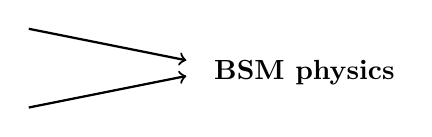
\begin{tikzpicture}
				\draw[-to,thick] (0,1) -- (2,0.6);
				\draw[-to,thick] (0,0) -- (2,0.4);
				\path (3.5,0.45) node {\textbf{BSM physics}};
			\end{tikzpicture}
		\end{textblock}
		\vspace{1cm}
		Higgs field:
		\begin{itemize}
			\item a complex doublet under SU(2)$_L$ symmetry group
			\item could be extended $\Rightarrow$ larger scalar sectors:
			\begin{itemize}
				\item Higgs sector
				\item additional structures $\Rightarrow$ \textbf{NEW BOSONS}
				\item new theory $\rightarrow$ 2HDM, SUSY
			\end{itemize} 
		\end{itemize}
		\vfill
	\end{frame}
		
	\begin{frame}{New spin-0 resonances analysis}
		\vfill
		\begin{center}
			BSM physics $\Rightarrow$ New spin-0 resonances search
		\end{center}
		\begin{itemize}
			\item \textbf{Channel}: $H \to \gamma\gamma$
			\item \textbf{Aim}: find an excess of events over\\ the expected background
			\item \textbf{Signal}:
			\begin{itemize}
				\item $X \to \gamma\gamma$ 
				\item a function of the resonance\\ mass $m_X$
				\item small SM assumptions
			\end{itemize}
			\item \textbf{Background}
			\begin{itemize}
				\item Non resonant background
				\begin{itemize}
					\item Irr $\to$ QCD di-photon\\ production
					\item Red $\to$ ($\gamma$,jet), (jet,jet)\\ with jet misidentification\\ (\textit{fake rate})
				\end{itemize}
				\item SM Higgs boson background
			\end{itemize}
		\end{itemize}
		\vfill 
		\begin{textblock}{1}(.45,.4)
			\includegraphics[width=.6\textwidth]{../thesis_images/HSM_prova.pdf}
		\end{textblock}
		\begin{textblock}{1.}(.2,.425)
			\begin{tikzpicture}
				\draw[-to,purple] (0,2.75) -- (6.5,0);
			\end{tikzpicture}
		\end{textblock}
		\begin{textblock}{1.}(.425,.6)
			\begin{tikzpicture}
				\draw[-to,yellow] (0,-.75) -- (1.5,0);
			\end{tikzpicture}
		\end{textblock}
		\begin{textblock}{1.}(.45,.7)
			\begin{tikzpicture}
				\draw[-to,blue] (0,-2) -- (2.3,0);
			\end{tikzpicture}
		\end{textblock}
	\end{frame}

	\begin{frame}{Events Selection}
		\vfill
		$H \to \gamma\gamma$ channel: \textbf{Event selected}
		\begin{itemize}
			\item $m_{\gamma\gamma}\ \epsilon\ [100,195]$ GeV
			\item two photons:
			\begin{itemize}
				\item identified
				\item isolation
				\item $p_T^{\gamma_1}/m_{\gamma\gamma}$ > 0.3 
				\item $p_T^{\gamma_2}/m_{\gamma\gamma}$ > 0.25
			\end{itemize}
			\item Fiducial events mimic selected events
		\end{itemize}
		\begin{textblock}{1}(.2,.2)
			\begin{table}[tbp]
				\centering
				\resizebox{7cm}{!}{
					\small
					\begin{tabular}{llcc}
						\toprule[1.5pt]
						Parameter									& Name						& Reconstruction Level	& Truth Level		\\
						\midrule
						$|\eta^{\gamma_i}|$							& $\eta$ cut				& $<2.37$ 				& $<2.37$			\\
						$p_T^{\gamma_1}/m_{\gamma\gamma}$			& Scalar relative $p_T$ cut & > 0.3					& > 0.3    			\\
						$p_T^{\gamma_2}/m_{\gamma\gamma}$			& Scalar relative $p_T$ cut & > 0.25				& > 0.25			\\
						$E_{T}^{cone20\ \gamma_i}/p_T^{\gamma_i}$ 	& Isolation cut 			& < 0.065				& < 0.065 			\\
						$p_{T}^{cone20\ \gamma_i}/p_T^{\gamma_i}$ 	& Isolation cut 			& < 0.05				& 		 			\\
						\bottomrule[1.5pt]
					\end{tabular}
				}
			\end{table}
		\end{textblock}
		\vspace{.5cm}
		\centering
		$\Downarrow$
		\begin{enumerate}\centering
			\item Categorisation
			\item Signal model
			\item Non-resonant background model
			\item SM Higgs boson background model
			\item Systematic uncertainties
			\item Expected results
		\end{enumerate}
		\vfill
	\end{frame}
	
	\begin{frame}{Categorisation}
		\vfill
		\begin{itemize}
			\item The events are classified into\\ mutually exclusive categories
			\item Designed to enhance the analysis\\ sensitivity
			\begin{itemize}
				\item maximise the signal and\\ bkg ratio $\frac{S}{B}$
				\item minimise the systematic\\ uncertainties
			\end{itemize}
			\item three categorisation test and\\ compared:
			\begin{itemize}
				\item $\gamma$ conversion status and\\ $\eta$ position cuts
				\item \texttt{Inclusive}, \texttt{catConvEta}, \texttt{catConv}
			\end{itemize}
		\end{itemize}
		\begin{textblock}{1}(.5,.15)
			\includegraphics[width=.5\textwidth]{../thesis_images/inclusive_tree.pdf}\\
			\includegraphics[width=.5\textwidth]{../thesis_images/catConvEta_tree.pdf}\\
			\includegraphics[width=.5\textwidth]{../thesis_images/catConv_tree.pdf}\\	
		\end{textblock}	
		\vfill
		\begin{textblock}{1.}(.25,.2)
			\begin{tikzpicture}
				\draw[-to,black!30] (0,-2.5) -- (3,0)
				node[below] {} -- (3,0)
				node[below] {} -- (3.35,3);
			\end{tikzpicture}
		\end{textblock}
		\begin{textblock}{1.}(.375,.435)
			\begin{tikzpicture}
				\draw[-to,black!30] (0,-1) -- (1,0)
				node[below] {} -- (2,2);
			\end{tikzpicture}
		\end{textblock}
		\begin{textblock}{1.}(.45,.68)
			\begin{tikzpicture}
				\draw[-to,black!30] (0,-0.75) -- (0.75,0);
			\end{tikzpicture}
		\end{textblock}
		\begin{textblock}{1}(0.,.85)
			\begin{figure}
				\resizebox{\textwidth}{!}{
					\begin{tikzpicture}[
						node distance = 0mm,
						start chain = going right,
						]
						\node[start=uibblue!80!black, scale=1] {Categories};
						\node[cont=gray!20!white,   scale=1] {Sig model};
						\node[cont=gray!20!white,   scale=1] {Bkg model};
						\node[cont=gray!20!white,   scale=1.1] {HSM model};
						\node[cont=gray!20!white,   scale=1] {Syst uncs};
						\node[cont=gray!20!white,   scale=1] {Exp results};
					\end{tikzpicture}		
				}
			\end{figure}
		\end{textblock}
	\end{frame}

	\begin{frame}{Signal model}
		\vfill
		For each categorisation:
		\begin{itemize}
			\item $\propto$ $m_X$
			\item \textbf{Function form}: \textit{Double-Sided Crystal\\ Ball} (DSCB):
			\begin{itemize}
				\item a gaussian core + power-law tails
				\item 6 parameters ($\mu, \sigma, a_{1,2}, p_{1,2}$)
			\end{itemize}
			\item \textbf{Samples}: \textit{ggF} MC samples with four\\ different resonance mass $m_X$ (110, 125,\\ 130 and GeV):
			\item \textbf{Fit}: a simultaneous DSCB fit:
			\begin{itemize}
				\item sensibility to new resonances
				\item DSCB parameters $\propto$ $m_X$:\\
				$par(m_X) = A^{par} + B^{par}\cdot m_X$
			\end{itemize}
		\end{itemize}
		\vspace{.5cm}
		\vfill
		\begin{textblock}{1}(.575,.1)
			\includegraphics[width=.45\textwidth]{../thesis_images/sigma_single.pdf}\\
			\includegraphics[width=.45\textwidth]{../thesis_images/PowhegPy8_NNLOPS_ggH125_catConvEta_no_fit.pdf}\\	
		\end{textblock}	
		\begin{textblock}{1}(0.,.85)
			\begin{figure}
				\resizebox{\textwidth}{!}{
					\begin{tikzpicture}[
						node distance = 0mm,
						start chain = going right,
						]
						\node[start=gray!20!white, scale=1] {Categories};
						\node[cont=uibblue!80!black,   scale=1] {Sig model};
						\node[cont=gray!20!white,   scale=1] {Bkg model};
						\node[cont=gray!20!white,   scale=1.1] {HSM model};
						\node[cont=gray!20!white,   scale=1] {Syst uncs};
						\node[cont=gray!20!white,   scale=1] {Exp results};
					\end{tikzpicture}		
				}
			\end{figure}
		\end{textblock}
	\end{frame}
	
	\begin{frame}{Signal model SM independence}
		\resizebox{.5\textwidth}{!}{
			\begin{box1}{Adolescenza}
				\begin{itemize}
					\item Compito evolutivo di sviluppo \\ $\Rightarrow$ costruzione identità personale\\
					$\Rightarrow$ garantisce integrità e unitarietà della persona
				\end{itemize}
			\end{box1}
		}\resizebox{.5\textwidth}{!}{
			\begin{box2}{Adolescenza e pandemia}
				\begin{itemize}
					\item Effetti a breve termine:
					\begin{itemize}
						\item aumento livelli di ansia, soprattutto nel genere femminile
						\item aumento sintomatologia depressiva
					\end{itemize}
				\end{itemize}
			\end{box2}
		}
		\begin{textblock}{1}(0.,.85)
			\begin{figure}
				\resizebox{\textwidth}{!}{
					\begin{tikzpicture}[
						node distance = 0mm,
						start chain = going right,
						]
						\node[start=gray!20!white, scale=1] {Categories};
						\node[cont=uibblue!80!black,   scale=1] {Sig model};
						\node[cont=gray!20!white,   scale=1] {Bkg model};
						\node[cont=gray!20!white,   scale=1.1] {HSM model};
						\node[cont=gray!20!white,   scale=1] {Syst uncs};
						\node[cont=gray!20!white,   scale=1] {Exp results};
					\end{tikzpicture}		
				}
			\end{figure}
		\end{textblock}
	\end{frame}
	
	\begin{frame}{Non-resonant background}
		\begin{textblock}{1}(0.,.85)
			\begin{figure}
				\resizebox{\textwidth}{!}{
					\begin{tikzpicture}[
						node distance = 0mm,
						start chain = going right,
						]
						\node[start=gray!20!white, scale=1] {Categories};
						\node[cont=gray!20!white,   scale=1] {Sig model};
						\node[cont=uibblue!80!black,   scale=1] {Bkg model};
						\node[cont=gray!20!white,   scale=1.1] {HSM model};
						\node[cont=gray!20!white,   scale=1] {Syst uncs};
						\node[cont=gray!20!white,   scale=1] {Exp results};
					\end{tikzpicture}		
				}
			\end{figure}
		\end{textblock}
	\end{frame}
	
	\begin{frame}{HSM background}
		\begin{textblock}{1}(0.,.85)
			\begin{figure}
				\resizebox{\textwidth}{!}{
					\begin{tikzpicture}[
						node distance = 0mm,
						start chain = going right,
						]
						\node[start=gray!20!white, scale=1] {Categories};
						\node[cont=gray!20!white,   scale=1] {Sig model};
						\node[cont=gray!20!white,   scale=1] {Bkg model};
						\node[cont=uibblue!80!black,   scale=1.1] {HSM model};
						\node[cont=gray!20!white,   scale=1] {Syst uncs};
						\node[cont=gray!20!white,   scale=1] {Exp results};
					\end{tikzpicture}		
				}
			\end{figure}
		\end{textblock}
	\end{frame}
\end{document}